\documentclass{article}

\usepackage{hyperref, graphicx}
\usepackage[scale = 0.9]{geometry}


\begin{document}
\section{BigQuery SQL}
\begin{itemize}
\item work with date
	\begin{itemize}
	\item \href{https://cloud.google.com/bigquery/docs/reference/standard-sql/date_functions#extract}{EXTRACT(DAY FROM date\_expression)}
	\end{itemize}
\item arithmatic operation with numeric data
\item \href{https://cloud.google.com/bigquery/docs/reference/standard-sql/string_functions}{string functions}
	\begin{itemize}
	\item check if contains ampersand sign: \verb|CONTAINS_SUBSTR(name, '&')|
	\item string append: \texttt{||}
	\end{itemize}
\end{itemize}

\section{command line}
\begin{itemize}
\item upload data to bucket (\verb|my_bucket|)
	\begin{itemize}
	\item upload a file to bucket: \verb|gsutil cp data1.csv gs://my_bucket|
	\item upload a folder to bucket: \verb|gsutil cp -r myfolder/ gs://my_bucket|
	\item list files in my bucket: \verb|gsutil ls gs://my_bucket|
	\end{itemize}
\item work with BigQuery (\verb|bq|)
	\begin{itemize}
	\item list datasets: \verb|bq ls|
	\item view a table in a database: \verb|bq show projectId:datasetId.tableId|
	\item run a query:
	\begin{verbatim}
	bq query --use_legacy_sql=false \
	'SELECT *
	FROM talbe'
	\end{verbatim}
	\end{itemize}
\item \href{https://1drv.ms/v/s!An3MvLGBA7qWjowPwVd8RAInk7_tDg?e=axGPRB}{BigQuery architecture}
	\begin{itemize}
	\item decoupling/denormolization of storage and compute. 
	BigQuery is based on a number of foundational technologies deployed in Google. Google has created a replicated distributed storage system that is based on a couple of systems. One is Colossus (globally distributed storage system) and Spanner (globally scalable relational database, for managing metadata about the data we store in BigQuery). The compute side is made up of two Google technologies. One is called Dremel which is a system that takes our SQL queries and breaks them down into distinct executable chunks and then produces the results based on those chunks and merges the results and delivers the results to us. Dremel does this by creating or deploying this work in jobs. A job is an abstraction for running a query or other operations within BigQuery. The system that manages jobs is known as Borg. Borg is a predecessor of Kubernetes. A lot of ideas that we're developed in Borg kind of influence the design of Kubernetes as well. \\

	Because the storage and the compute are separated. It's really important that we're able to quickly move data between storage and compute. And that's done using the Jupiter network. Jupiter network is network hardware that provides for petabit scale throughput and it is a key to successfully decoupling storage and compute. 
	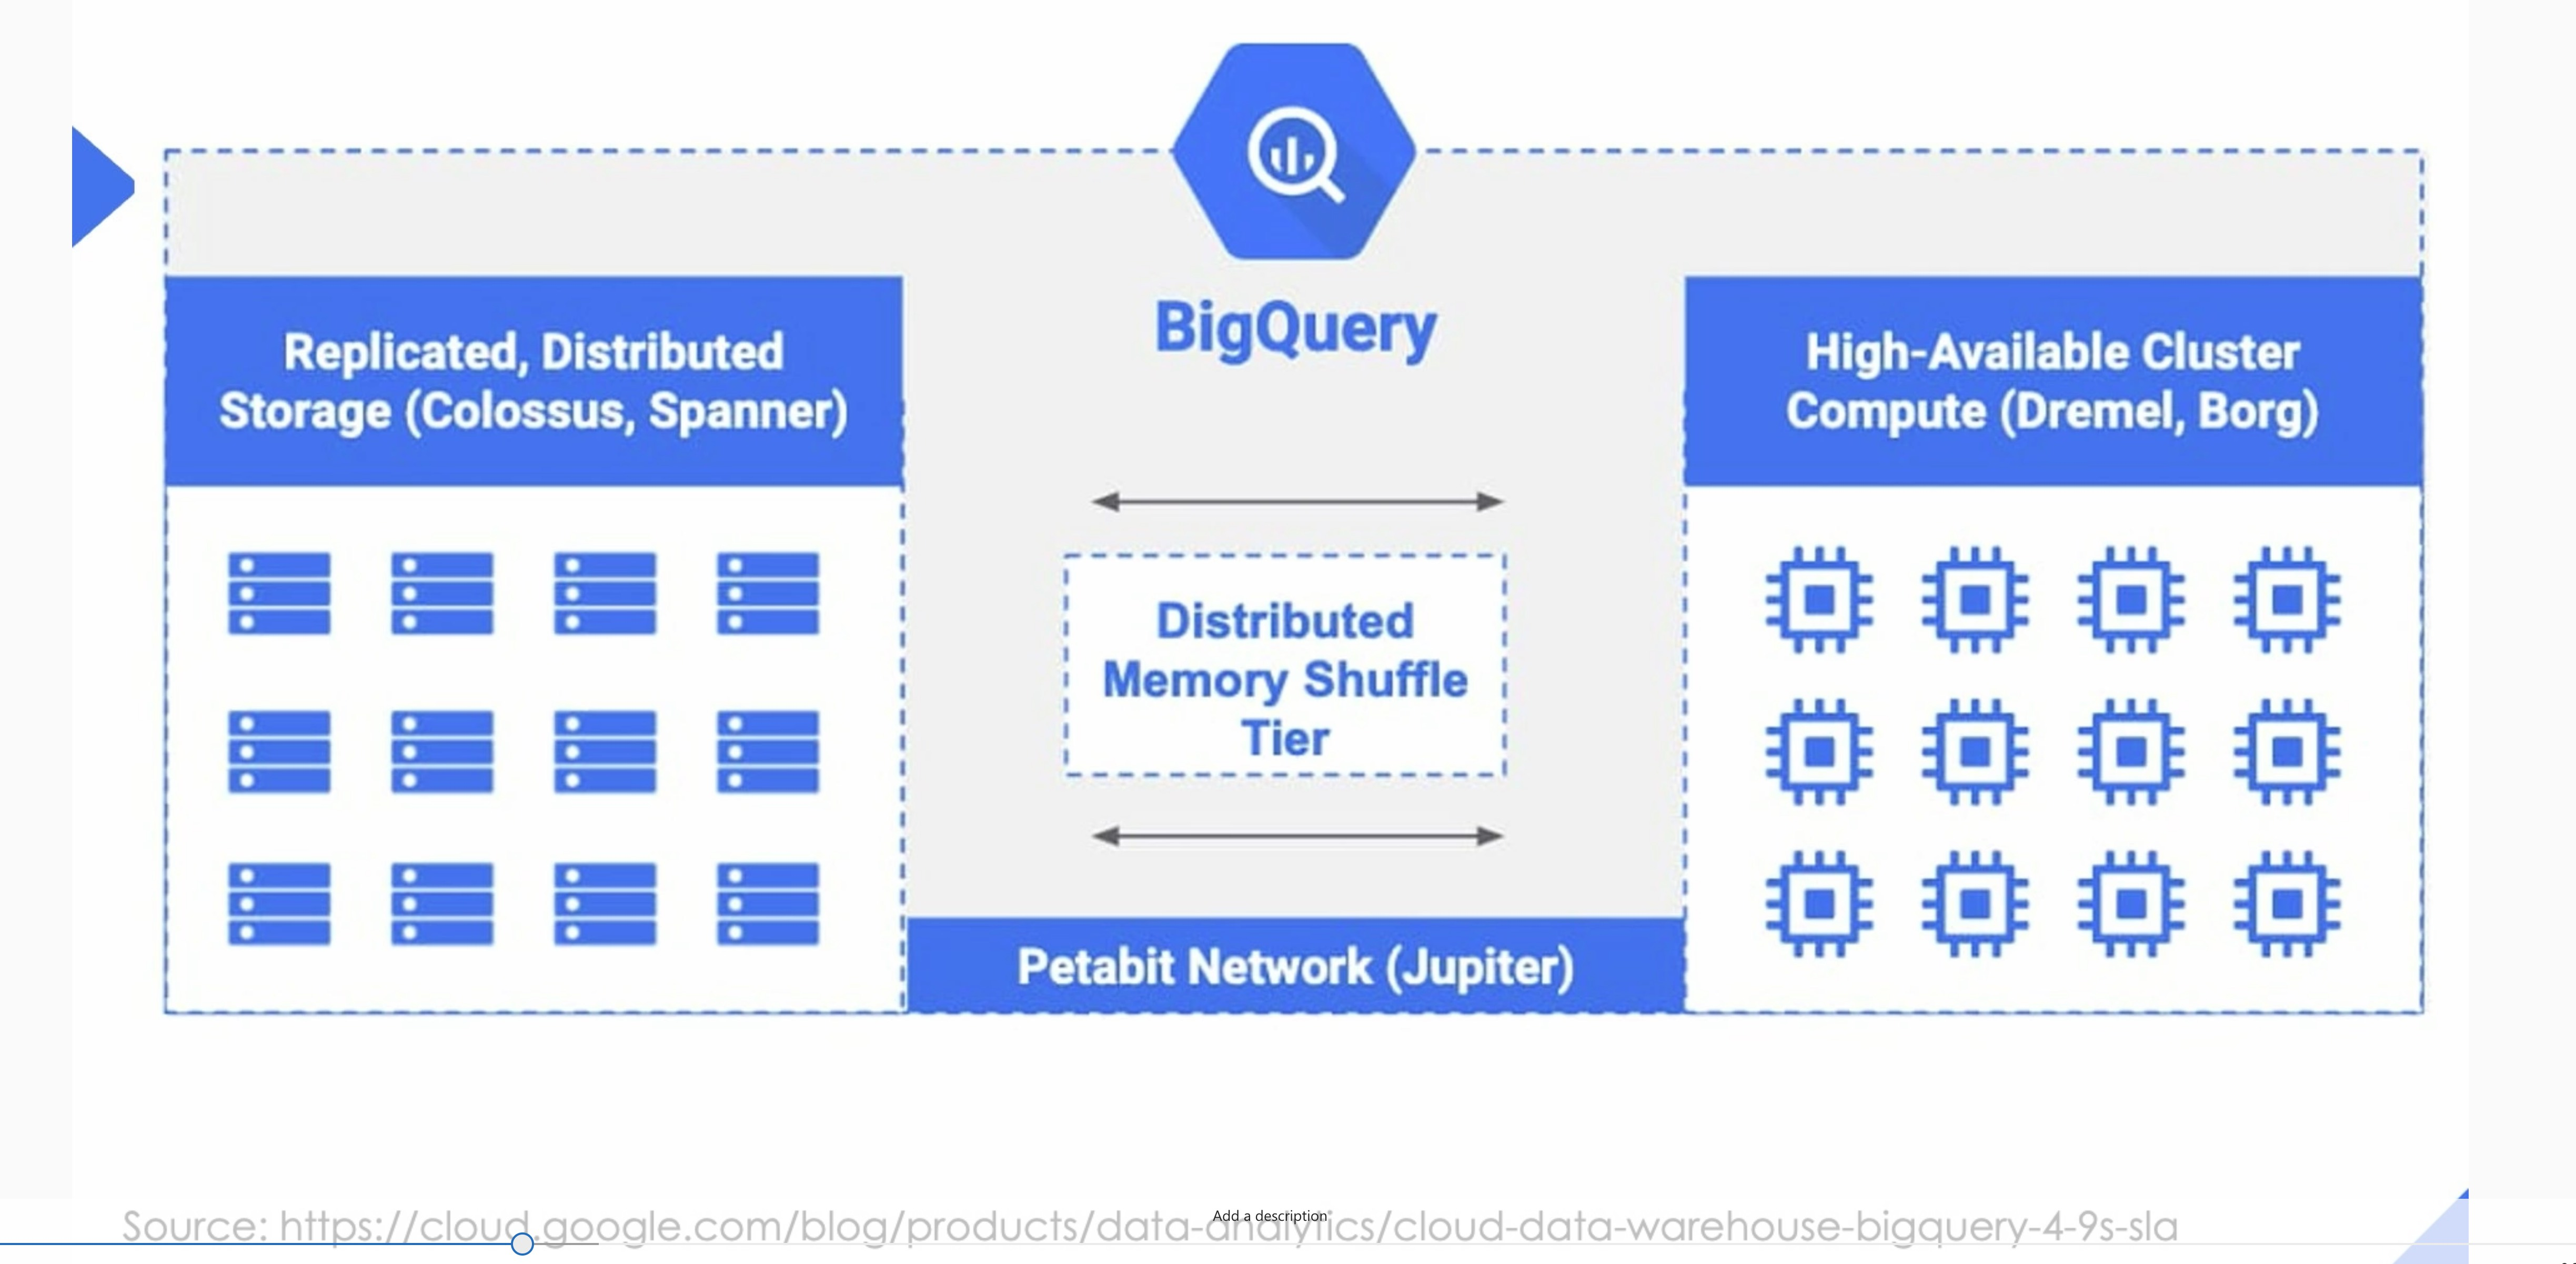
\includegraphics[width= 0.7\textwidth]{figure1.jpg}

	
	\end{itemize}
\end{itemize}

\end{document}